\documentclass[12pt,a4paper]{report}

\usepackage[top=2.5cm, bottom=2.5cm, left=3.5cm, right=2.5cm]{geometry}
\usepackage{setspace}
\setstretch{1.3}
\setlength{\parskip}{2.5pt}
\setlength{\parindent}{1.0cm}
\widowpenalty=10000
\clubpenalty=10000

\usepackage{amsmath}
\usepackage{amssymb}
\usepackage{amsfonts}
\usepackage{algorithm}
\usepackage{algpseudocode}
\floatname{algorithm}{Thuật toán}
\numberwithin{algorithm}{chapter}
\renewcommand{\algorithmicrequire}{\textbf{Đầu vào:}}
\renewcommand{\algorithmicensure}{\textbf{Đầu ra:}}

\usepackage{fontspec}
\setmainfont{Times New Roman}
\setmonofont{Consolas}[Scale=MatchLowercase]

\usepackage{graphicx}
\graphicspath{{../}}
\usepackage{float}
\usepackage{placeins}
\usepackage{fancybox}
\usepackage{array}
\usepackage{booktabs}
\usepackage{longtable}
\usepackage{tabularx}
\usepackage{enumitem}
\usepackage{xcolor}
\usepackage{hyperref}
\usepackage{fancyhdr}
\usepackage{titlesec}
\usepackage{titletoc}
\usepackage{chngcntr}

% Đánh số toàn cục liên tục cho Bảng và Hình theo chuẩn mẫu báo cáo thực tập
\counterwithout{table}{chapter}
\counterwithout{figure}{chapter}

% Định nghĩa hệ số đếm: Chương dùng số La Mã, Mục và Tiểu mục dùng số Ả Rập
\renewcommand{\thechapter}{\Roman{chapter}}
\renewcommand{\thesection}{\arabic{chapter}.\arabic{section}}
\renewcommand{\thesubsection}{\arabic{chapter}.\arabic{section}.\arabic{subsection}}

% Cấu hình tiêu đề theo Chuẩn Báo cáo Thực tập Công nghiệp (Báo-cáo-thực-tập-CN.pdf)
\titleformat{\chapter}[block]
    {\normalfont\large\bfseries\centering}
    {CHƯƠNG \thechapter:\quad}
    {0pt}
    {}
\titleformat{name=\chapter,numberless}[hang]
    {\normalfont\large\bfseries\centering}
    {}
    {0pt}
    {}
\titlespacing*{\chapter}
    {0pt}
    {-20pt}
    {15pt}

\titleformat{\section}[hang]
    {\normalfont\large\bfseries}
    {\thesection.\quad}
    {0pt}
    {}
\titlespacing*{\section}
    {0pt}
    {12pt}
    {6pt}

\titleformat{\subsection}[hang]
    {\normalfont\normalsize\bfseries\itshape}
    {\thesubsection.\quad}
    {0pt}
    {}
\titlespacing*{\subsection}
    {0pt}
    {10pt}
    {4pt}

% Cấu hình hiển thị Mục lục (TOC) theo chuẩn mẫu trường: CHƯƠNG I: <TÊN CHƯƠNG>
\titlecontents{chapter}[0pt]
    {\vspace{3pt}\bfseries}
    {CHƯƠNG \thecontentslabel:\quad}
    {}
    {\quad\titlerule*[0.75pc]{.}\contentspage}

\titlecontents{section}[2.2em]
    {\normalfont}
    {\thecontentslabel.\quad}
    {}
    {\quad\titlerule*[0.75pc]{.}\contentspage}

\titlecontents{subsection}[4.5em]
    {\normalfont\itshape}
    {\thecontentslabel.\quad}
    {}
    {\quad\titlerule*[0.75pc]{.}\contentspage}

% Cấu hình hiển thị Danh mục Bảng biểu & Hình ảnh với tiền tố Bảng X: và Hình X:
\titlecontents{table}[0pt]
    {\normalfont}
    {Bảng \thecontentslabel:\quad}
    {}
    {\quad\titlerule*[0.75pc]{.}\contentspage}

\titlecontents{figure}[0pt]
    {\normalfont}
    {Hình \thecontentslabel:\quad}
    {}
    {\quad\titlerule*[0.75pc]{.}\contentspage}

\usepackage{tikz}
\usetikzlibrary{
    arrows.meta,
    backgrounds,
    calc,
    fit,
    positioning,
    shapes.geometric,
    shapes.multipart
}

\renewcommand{\contentsname}{MỤC LỤC}
\renewcommand{\listfigurename}{DANH MỤC HÌNH ẢNH}
\renewcommand{\listtablename}{DANH MỤC BẢNG BIỂU}
\renewcommand{\chaptername}{Chương}
\renewcommand{\figurename}{Hình}
\renewcommand{\tablename}{Bảng}
\renewcommand{\bibname}{TÀI LIỆU THAM KHẢO}

\hypersetup{
    colorlinks=true,
    linkcolor=black,
    urlcolor=black,
    citecolor=black
}
\urlstyle{same}

\setlist[itemize]{label={-}, leftmargin=1.0cm, itemsep=2pt, topsep=2pt, parsep=0pt}
\setlist[enumerate]{leftmargin=1.0cm, itemsep=2pt, topsep=2pt, parsep=0pt}
\renewcommand{\arraystretch}{1.25}
\setlength{\tabcolsep}{3pt}
\newcolumntype{L}[1]{>{\raggedright\hspace{0pt}\arraybackslash}p{#1}}
\newcolumntype{Y}{>{\raggedright\hspace{0pt}\arraybackslash}X}
\newcommand{\code}[1]{{\ttfamily\urlstyle{same}\nolinkurl{#1}}}

% Quy chuẩn mẫu trường: TUYỆT ĐỐI KHÔNG DÙNG RUNNING HEADER VÀ ĐƯỜNG KẺ Ở ĐỈNH TRANG
\pagestyle{plain}
\fancypagestyle{plain}{
    \fancyhf{}
    \fancyfoot[C]{\thepage}
    \renewcommand{\headrulewidth}{0pt}
}

\setlength{\headheight}{16.5pt}
\emergencystretch=3em
\hyphenation{RareProtSelect Subfamily Subfamilies Peptidase Peptidases Facility Location BLASTp}
\renewcommand{\topfraction}{0.90}
\renewcommand{\bottomfraction}{0.80}
\renewcommand{\textfraction}{0.07}
\renewcommand{\floatpagefraction}{0.85}
\setcounter{topnumber}{3}
\setcounter{bottomnumber}{2}
\setcounter{totalnumber}{4}

\begin{document}

% 1. Trang bìa: không số trang, không running header
\pagenumbering{gobble}
\thispagestyle{empty}
\thisfancypage{\setlength{\fboxsep}{0.2cm}\setlength{\fboxrule}{1pt}\doublebox}{}
\begin{titlepage}
    \thispagestyle{empty}
    \begin{center}
        \large
        \textbf{BỘ GIÁO DỤC VÀ ĐÀO TẠO}\\
        \textbf{ĐẠI HỌC PHENIKAA}\\
        \vspace{-0.9em}
        \rule{3cm}{0.4pt}
    \end{center}

    \vspace{0.3cm}
    \begin{center}
        
\includegraphics[height=2.8cm]{Images/pnk_logo.jpg}
    \end{center}

    \vspace{0.3cm}
    \begin{center}
        {\fontsize{19pt}{23pt}\selectfont\textbf{BÁO CÁO THỰC TẬP CÔNG NGHIỆP}\par}
        \vspace{0.6cm}
        {\fontsize{13pt}{17pt}\selectfont\textbf{TÊN ĐỀ TÀI}\par}
        \vspace{0.3cm}
        {\fontsize{15pt}{19pt}\selectfont\textbf{CHỌN TẬP PROTEIN ĐẠI DIỆN\\CÓ ƯU TIÊN NHÓM HIẾM\\BẰNG TỐI ƯU HÓA SUBMODULAR}\par}
    \end{center}

    \vspace{0.8cm}
    \begin{center}
        \begin{tabular}{@{}p{7.2cm}l@{}}
            \multicolumn{2}{@{}l@{}}{\textbf{Sinh viên:} Đoàn Anh Hùng} \\
            \textbf{Mã số sinh viên:} 23010022 & \textbf{Khóa:} K17 \\
            \textbf{Ngành:} Khoa học máy tính tài năng & \textbf{Hệ:} Đại học chính quy \\
            \multicolumn{2}{@{}l@{}}{\textbf{Cơ sở thực tập:} Phòng thí nghiệm Tối ưu hóa các hệ thống lớn (ORLab)} \\
            \multicolumn{2}{@{}l@{}}{\textbf{Giảng viên hướng dẫn:} TS. Trần Đình Tân}
        \end{tabular}
    \end{center}

    \vspace*{\fill}
    \begin{center}
        \textbf{Hà Nội - Năm 2026}
    \end{center}
\end{titlepage}

\clearpage

% 2. Phiếu nhận xét chuẩn mẫu Báo-cáo-thực-tập-CN.pdf: 1 trang duy nhất, không số trang
\thispagestyle{empty}
\thispagestyle{empty}
\phantomsection

\begin{center}
    \vspace*{0.2cm}
    {\Large\textbf{NHẬN XÉT BÁO CÁO THỰC TẬP CÔNG NGHIỆP}}\par
    \vspace{0.8cm}
\end{center}

\begingroup
\setstretch{1.0}
\setlength{\parskip}{0pt}
\noindent\makebox[\linewidth]{\dotfill}\par\vspace{0.40cm}
\noindent\makebox[\linewidth]{\dotfill}\par\vspace{0.40cm}
\noindent\makebox[\linewidth]{\dotfill}\par\vspace{0.40cm}
\noindent\makebox[\linewidth]{\dotfill}\par\vspace{0.40cm}
\noindent\makebox[\linewidth]{\dotfill}\par\vspace{0.40cm}
\noindent\makebox[\linewidth]{\dotfill}\par\vspace{0.40cm}
\noindent\makebox[\linewidth]{\dotfill}\par\vspace{0.40cm}
\noindent\makebox[\linewidth]{\dotfill}\par\vspace{0.40cm}
\noindent\makebox[\linewidth]{\dotfill}\par\vspace{0.40cm}
\noindent\makebox[\linewidth]{\dotfill}\par\vspace{0.40cm}
\noindent\makebox[\linewidth]{\dotfill}\par\vspace{0.40cm}
\noindent\makebox[\linewidth]{\dotfill}\par\vspace{0.40cm}
\noindent\makebox[\linewidth]{\dotfill}\par\vspace{0.40cm}
\noindent\makebox[\linewidth]{\dotfill}\par\vspace{0.40cm}
\noindent\makebox[\linewidth]{\dotfill}\par\vspace{0.40cm}
\noindent\makebox[\linewidth]{\dotfill}\par\vspace{0.40cm}
\noindent\makebox[\linewidth]{\dotfill}\par\vspace{0.40cm}
\noindent\makebox[\linewidth]{\dotfill}\par\vspace{0.40cm}
\noindent\makebox[\linewidth]{\dotfill}\par\vspace{0.40cm}
\noindent\makebox[\linewidth]{\dotfill}\par\vspace{0.40cm}
\noindent\makebox[\linewidth]{\dotfill}\par\vspace{0.40cm}
\noindent\makebox[\linewidth]{\dotfill}
\endgroup

\clearpage

\clearpage

% 3. Lời cảm ơn: không số trang
\thispagestyle{empty}
\thispagestyle{empty}
\phantomsection

\begin{center}
    \vspace*{0.2cm}
    {\Large\textbf{LỜI CẢM ƠN}}\par
    \vspace{0.8cm}
\end{center}

Lời đầu tiên, tôi xin bày tỏ lòng biết ơn chân thành và sâu sắc nhất tới Phòng thí nghiệm Tối ưu hóa các hệ thống lớn (ORLab) cùng TS. Trần Đình Tân đã tiếp nhận, tạo điều kiện thuận lợi, tận tình hướng dẫn và định hướng nghiên cứu cho tôi trong suốt thời gian thực tập công nghiệp tại Lab.

Nhờ sự hướng dẫn sát sao của thầy cùng các anh chị nghiên cứu viên tại ORLab, tôi đã được tiếp cận trực tiếp với các bài toán tối ưu hóa tổ hợp thực tế, đặc biệt là lý thuyết tối ưu hóa hàm submodular kết hợp cùng mô hình ngôn ngữ protein ESM-2. Môi trường nghiên cứu chuyên nghiệp, bài bản và học thuật tại ORLab đã giúp tôi rèn luyện tư duy phản biện, kỹ năng giải quyết vấn đề và năng lực triển khai mã nguồn trên các hệ thống tính toán hiệu năng cao.

Tôi cũng xin trân trọng gửi lời cảm ơn tới Ban giám hiệu Trường Đại học Phenikaa cùng các thầy cô giáo Khoa Công nghệ thông tin đã nhiệt tình giảng dạy, truyền đạt những kiến thức nền tảng vững chắc để tôi có thể hoàn thành tốt đợt thực tập này.

\vspace{1.5cm}
\begin{flushright}
    \textit{Hà Nội, tháng 11 năm 2026}\\
    \textbf{Ký tên}\\
    \vspace{2.0cm}
    \textbf{Đoàn Anh Hùng}
\end{flushright}

\clearpage

\clearpage

% 4. Mục lục: không số trang, vừa vặn trên 1 trang duy nhất
\thispagestyle{empty}
\begingroup
\setstretch{0.90}
\setlength{\parskip}{0pt}
\addtocontents{toc}{\protect\thispagestyle{empty}}
\addtocontents{toc}{\protect\enlargethispage{2.5\baselineskip}}
\tableofcontents
\endgroup
\clearpage

% 5. Danh mục bảng biểu & Danh mục hình ảnh: gộp trên cùng 1 trang duy nhất, không số trang
\thispagestyle{empty}
\begingroup
\setstretch{1.0}
\setlength{\parskip}{0pt}
{\centering\Large\bfseries DANH MỤC BẢNG BIỂU\par\vspace{0.4cm}}
\makeatletter
\let\orig@addvspace\addvspace
\renewcommand*{\addvspace}[1]{}
\@starttoc{lot}
\vspace{1.2cm}
{\centering\Large\bfseries DANH MỤC HÌNH ẢNH\par\vspace{0.4cm}}
\@starttoc{lof}
\let\addvspace\orig@addvspace
\makeatother
\endgroup
\clearpage

% 6. Thân bài 5 chương chuẩn Báo cáo Thực tập Công nghiệp: Đánh số trang Ả Rập từ 1
\pagenumbering{arabic}
\setcounter{page}{1}
\pagestyle{plain}

\chapter{GIỚI THIỆU ĐƠN VỊ THỰC TẬP}
\label{chap:gioi_thieu_orlab}

Phòng thí nghiệm Tối ưu hóa các hệ thống lớn (ORLab) trực thuộc Trường Đại học Phenikaa là đơn vị nghiên cứu học thuật chuyên sâu trong hai lĩnh vực mũi nhọn: tối ưu hóa và trí tuệ nhân tạo. Với phương châm kết hợp chặt chẽ giữa lý thuyết toán học giải tích và triển khai kỹ thuật hiệu năng cao, ORLab đóng vai trò tiên phong trong việc phát triển các mô hình tính toán hiện đại để giải quyết các bài toán thực tiễn phức tạp có quy mô dữ liệu lớn.

\section{Thông tin chung về cơ sở thực tập}
\label{sec:thong_tin_chung_orlab}

Các thông tin định danh chính thức của phòng thí nghiệm được công bố trên cổng thông tin khoa học của Lab tại địa chỉ \url{https://www.orlab.vn/} bao gồm:

\begin{itemize}
    \item \textbf{Tên đơn vị}: Phòng thí nghiệm Tối ưu hóa các hệ thống lớn (ORLab).
    \item \textbf{Trưởng phòng thí nghiệm}: PGS.TS. Phạm Văn Cảnh.
    \item \textbf{Cán bộ hướng dẫn nghiên cứu}: TS. Trần Đình Tân.
    \item \textbf{Trụ sở làm việc}: phòng 2211, tầng 22 tòa nhà A9, Trường Đại học Phenikaa, đường Nguyễn Trác, phường Dương Nội, Hà Nội, Việt Nam.
    \item \textbf{Website chính thức}: \url{https://www.orlab.vn/}
\end{itemize}

\begin{figure}[htbp!]
    \centering
    
\includegraphics[width=0.24\textwidth]{Images/orlab/orlab_logo.png}
    \caption[Logo phòng thí nghiệm ORLab]{Logo chính thức của phòng thí nghiệm ORLab.}
    \label{fig:orlab_logo}
\end{figure}

\section{Lịch sử hình thành và sứ mệnh phát triển}
\label{sec:lich_su_orlab}

Được thành lập tại Trường Đại học Phenikaa, ORLab định vị sứ mệnh trở thành trung tâm nghiên cứu xuất sắc về vận trù học, giải thuật tối ưu và ứng dụng trí tuệ nhân tạo. Phòng thí nghiệm tập trung giải quyết các bài toán tối ưu tổ hợp phức tạp thuộc lớp NP-khó xuất hiện trong giao thông vận tải, logistics, chuỗi cung ứng công nghiệp và khoa học sự sống.

Môi trường học thuật tại ORLab đề cao tính chính xác toán học, phương pháp luận thực nghiệm khách quan và khả năng hiện thực hóa thuật toán trên các hệ thống tính toán phân tán và tăng tốc phần cứng. Sinh viên và học viên cao học khi tham gia nghiên cứu tại Lab được rèn luyện quy trình làm việc khoa học chuẩn mực quốc tế: từ khâu phân tích bài toán, xây dựng mô hình giải tích, chứng minh các tính chất cận xấp xỉ, đến khâu thiết kế pipeline thử nghiệm và công bố kết quả.

\section{Cơ cấu tổ chức và nhân sự nghiên cứu}
\label{sec:co_cau_orlab}

Cơ cấu nhân sự của ORLab quy tụ các nhà khoa học giàu kinh nghiệm, các tiến sĩ tốt nghiệp từ các trường đại học uy tín trong và ngoài nước, cùng lực lượng nghiên~cứu~sinh~và~sinh~viên~tài~năng:

\begin{figure}[htbp!]
    \centering
    \begin{minipage}{0.45\textwidth}
        \centering
        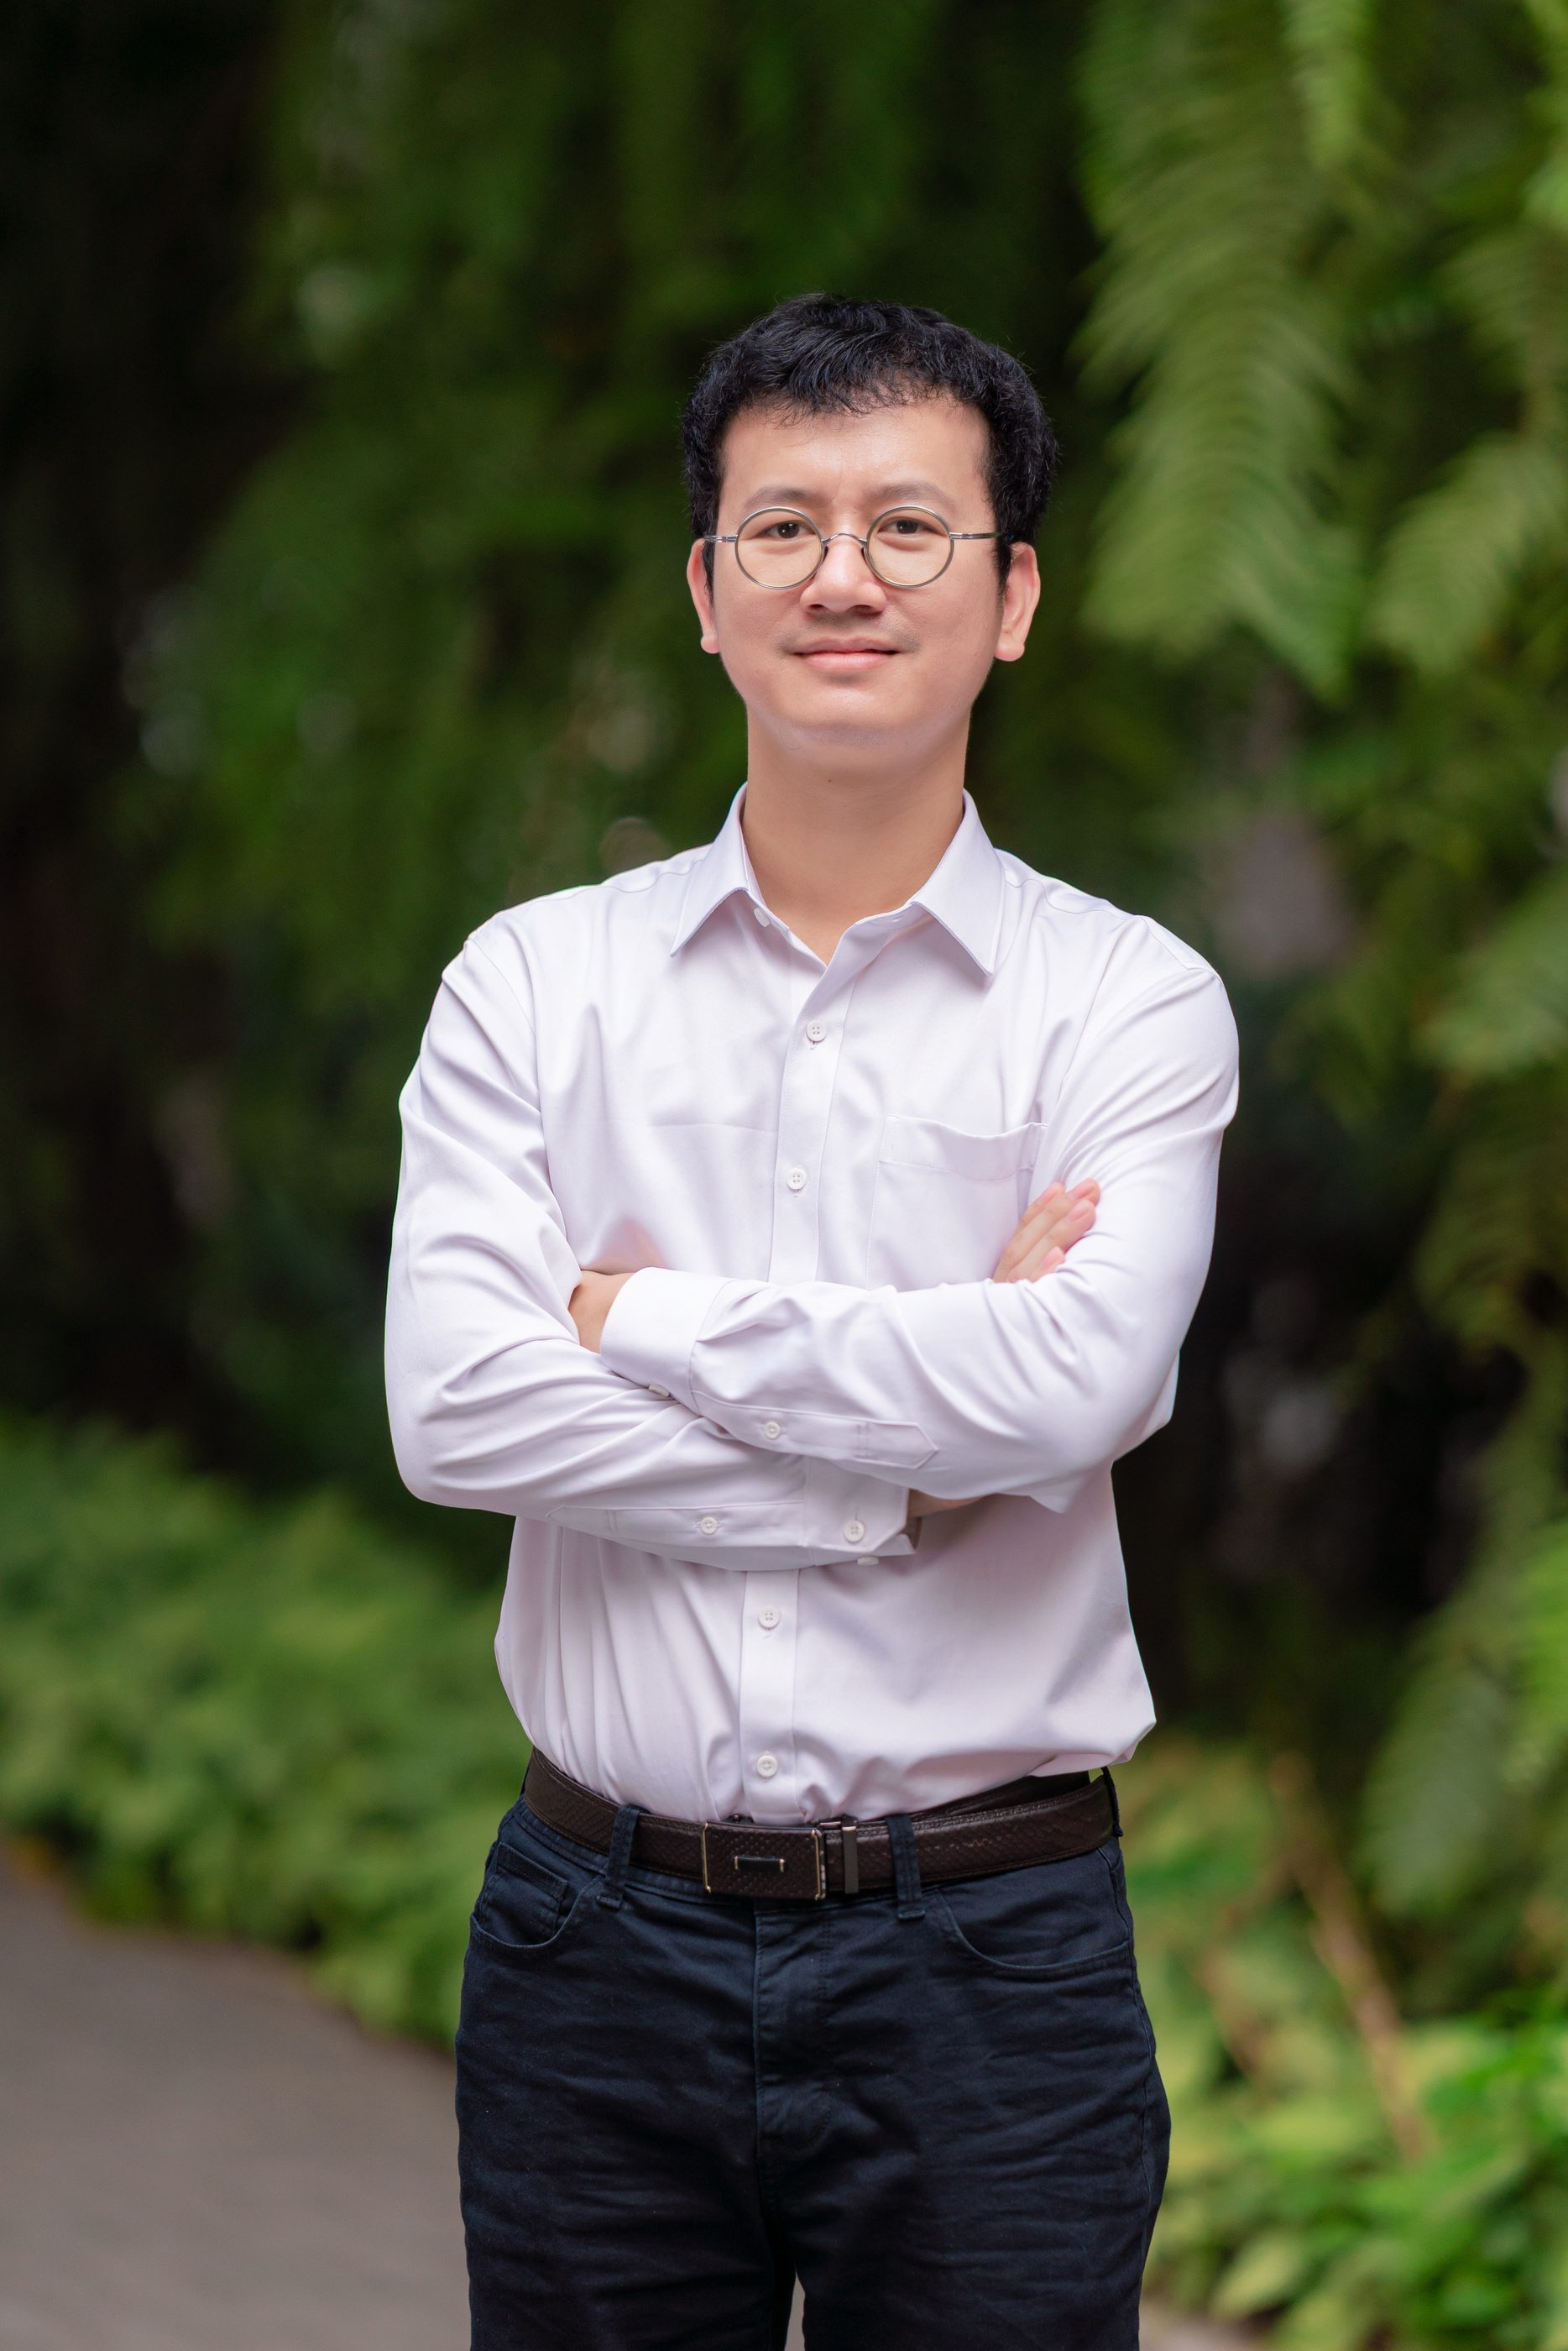
\includegraphics[width=0.34\textwidth,height=4.6cm,keepaspectratio]{Images/orlab/phamvancanh.jpg}\par
        \vspace{2pt}
        \textbf{PGS.TS. Phạm Văn Cảnh}\\
        \textit{Trưởng phòng thí nghiệm}
    \end{minipage}
    \hfill
    \begin{minipage}{0.45\textwidth}
        \centering
        
\includegraphics[width=0.34\textwidth,height=4.6cm,keepaspectratio]{Images/orlab/trandinhtan.jpg}\par
        \vspace{2pt}
        \textbf{TS. Trần Đình Tân}\\
        \textit{Cán bộ hướng dẫn}
    \end{minipage}
    \vspace{2pt}
    \caption{Lãnh đạo và cán bộ hướng dẫn khoa học tại phòng thí nghiệm ORLab.}
    \label{fig:orlab_leadership}
\end{figure}

\begin{itemize}
    \item \textbf{Trưởng phòng thí nghiệm}: PGS.TS. Phạm Văn Cảnh chịu trách nhiệm định hướng chiến lược học thuật tổng thể, chủ trì các đề tài khoa học trọng điểm và kết nối hợp tác quốc tế.
    \item \textbf{Cán bộ nghiên cứu và hướng dẫn}: TS. Trần Đình Tân trực tiếp định hướng chuyên môn, giao nhiệm vụ nghiên cứu và đồng hành cùng tôi trong suốt quá trình triển khai đề tài thực tập.
    \item \textbf{Thành viên nghiên cứu chủ chốt}: Các giảng viên và nhà nghiên cứu như TS. Dương Thị Kim Huyền, TS. Hà Thị Kim Dung, TS. Tạ Thúy Anh, cùng các nghiên cứu sinh tiến sĩ tích cực trao đổi học thuật và hỗ trợ kỹ thuật chuyên sâu.
    \item \textbf{Nhóm sinh viên nghiên cứu}: Trực tiếp hiện thực hóa giải thuật, chạy các kịch bản thực nghiệm trên máy chủ GPU và xây dựng báo cáo khoa học.
\end{itemize}

\section{Các hướng nghiên cứu chính của đơn vị}
\label{sec:cac_huong_nghien_cuu_orlab}

Theo định hướng chính thức từ cổng thông tin ORLab, hoạt động nghiên cứu của phòng thí nghiệm được tổ chức thành hai hướng nghiên cứu chính:

\begin{enumerate}[itemsep=1pt, parsep=0pt, topsep=2pt]
    \item \textbf{Hướng nghiên cứu 01: Tối ưu hóa}:
    \begin{itemize}[itemsep=1pt, parsep=0pt, topsep=1pt]
        \item \textit{Tối ưu hóa tổ hợp}: Phát triển các thuật toán chính xác và thuật toán xấp xỉ cho các bài toán tối ưu trên đồ thị và mạng lưới.
        \item \textit{Tối ưu hóa hàm submodular}: Khai thác tính chất suy giảm cận biên để giải quyết hiệu quả bài toán chọn tập con đại diện, nén dữ liệu và bài toán Facility Location với bảo đảm cận xấp xỉ lý thuyết.
        \item \textit{Định tuyến và lập lịch}: Ứng dụng giải quyết bài toán điều vận phương tiện VRP, lập lịch sản xuất công nghiệp và tối ưu chuỗi cung ứng.
        \item \textit{Tối ưu hóa ngẫu nhiên và bền vững}: Xây dựng các mô hình tối ưu có khả năng chống chịu nhiễu và biến động dữ liệu thực tế.
    \end{itemize}
    \item \textbf{Hướng nghiên cứu 02: Trí tuệ nhân tạo}:
    \begin{itemize}[itemsep=1pt, parsep=0pt, topsep=1pt]
        \item \textit{Học máy và học sâu}: Xây dựng các kiến trúc mô hình học biểu diễn dữ liệu quy mô lớn.
        \item \textit{Học tăng cường}: Ứng dụng trong việc tự động hóa quá trình ra quyết định và điều khiển thông minh.
        \item \textit{Học liên kết}: Bảo mật dữ liệu phân tán trong huấn luyện mô hình.
        \item \textit{Mô hình ngôn ngữ lớn và hệ thống đa tác tử}: Nghiên cứu cơ chế phối hợp tác tử tự trị và ứng dụng mô hình ngôn ngữ lớn vào giải quyết các bài~toán~phức~tạp.
    \end{itemize}
\end{enumerate}

\section{Sự chuẩn bị của tôi cho kỳ thực tập công nghiệp}
\label{sec:chuan_bi_thuc_tap}

Để đáp ứng các yêu cầu nghiên cứu khắt khe và hoàn thành tốt nhiệm vụ được giao tại phòng thí nghiệm ORLab, tôi đã chủ động chuẩn bị đầy đủ cả về kiến thức chuyên môn lẫn kỹ~năng~thực~hành:

\subsection{Về cơ sở thực tập}
Tôi đã chủ động tìm hiểu các công trình khoa học đã công bố của ORLab, theo dõi thông tin trên website của Lab, tham gia các buổi seminar học thuật và liên hệ trực tiếp với TS. Trần Đình Tân để được tiếp nhận vào nhóm nghiên cứu về tối ưu hóa chọn tập protein đại~diện một cách hiệu quả.

\subsection{Về kiến thức và kỹ năng kỹ thuật}
Tôi đã củng cố vững chắc các nền tảng công nghệ phục vụ trực tiếp cho đề tài nghiên cứu:
\begin{itemize}[itemsep=1pt, parsep=0pt, topsep=2pt]
    \item \textbf{Nền tảng toán học}: Ôn tập đại số tuyến tính, lý thuyết đồ thị, giải tích ma trận và lý thuyết tối ưu hóa hàm submodular có ràng buộc lực lượng.
    \item \textbf{Kỹ năng lập trình chuyên nghiệp}: Sử dụng thành thạo Python 3.12, trình quản lý môi trường hiện đại uv, cùng các thư viện khoa học lõi gồm PyTorch, Biopython, NumPy, SciPy và Scikit-learn.
    \item \textbf{Kỹ thuật tăng tốc phần cứng}: Nắm vững kỹ thuật lập trình vector hóa trên GPU CUDA nhằm tính toán song song ma trận tương đồng kích thước lớn với tốc độ và hiệu năng cao.
\end{itemize}

\chapter{MỤC TIÊU, KẾ HOẠCH VÀ LỊCH TRÌNH}
\label{chap:ke_hoach_lich_trinh}

Việc xác định mục tiêu rõ ràng và thiết lập kế hoạch làm việc tuần tự đóng vai trò tiên quyết nhằm bảo đảm tiến độ nghiên cứu và chất lượng sản phẩm bàn giao tại ORLab. Trong chương này, các mục tiêu thực tập, bảng phân bổ công việc theo giai đoạn và lịch trình triển khai chi tiết theo tuần được trình bày cụ thể.

\section{Mục tiêu thực tập}
\label{sec:muc_tieu_thuc_tap}

Quá trình thực tập tại phòng thí nghiệm ORLab được thiết kế nhằm hoàn thiện đồng thời hai nhóm mục tiêu cốt~lõi:

\subsection{Mục tiêu cá nhân}
\begin{itemize}[noitemsep,topsep=2pt]
    \item Thích nghi với quy trình làm việc học thuật chuyên nghiệp, phương pháp tư duy nghiên cứu khoa học độc lập và tác phong kỷ luật của một phòng thí nghiệm nghiên cứu hiện đại.
    \item Nâng cao năng lực giải quyết các bài toán tối ưu NP-khó trong thực tiễn thông qua việc xây dựng mô hình toán học giải tích chặt chẽ.
    \item Hoàn thành xuất sắc học phần thực tập công nghiệp với báo cáo kỹ thuật và nghiệm thu thực nghiệm đầy đủ.
\end{itemize}

\subsection{Mục tiêu nghề nghiệp}
\begin{itemize}[noitemsep,topsep=2pt]
    \item Làm chủ kỹ năng phát triển phần mềm nghiên cứu khoa học Research Software Engineering với công cụ quản lý môi trường hiện đại uv và ngôn ngữ Python 3.12.
    \item Tích lũy kinh nghiệm xử lý dữ liệu lớn trong tin sinh học phân tử, bao gồm cấu trúc tệp FASTA, chuẩn hóa mã phân loại MEROPS và trích xuất vector đặc trưng từ mô hình ngôn ngữ protein ESM-2.
    \item Định hướng phát triển sự nghiệp theo con đường kỹ sư nghiên cứu trí tuệ nhân tạo và giải thuật tối ưu.
\end{itemize}

\clearpage
\section{Kế hoạch thực tập tại cơ sở}
\label{sec:ke_hoach_thuc_tap}

\subsection{Nội dung công việc được giao}
Tại ORLab, tôi được giao nghiên cứu đề tài \textbf{``Chọn tập protein đại diện có ưu tiên nhóm hiếm bằng tối ưu hóa submodular mang tên RareProtSelect''}, với 4 nhiệm vụ cốt lõi:
\begin{enumerate}
    \item Nghiên cứu bài báo nền tảng về lựa chọn chuỗi protein đại diện bằng hàm submodular Facility Location và chỉ ra hạn chế của phương pháp hiện có đối với phân bố mất cân bằng quy mô nhóm.
    \item Đề xuất mô hình toán học mới tích hợp hàm trọng số phạt quy mô nhóm và kết hợp không gian tương đồng BLASTp với vector nhúng ngữ nghĩa ESM-2.
    \item Thiết kế và cài đặt pipeline tính toán hoàn chỉnh, bao gồm thuật toán tham lam cắt tỉa Pruned Greedy 90\% tăng tốc trên GPU và cơ chế tổng hợp thứ~hạng~toàn~cục.
    \item Đo đạc thực nghiệm định lượng trên tập dữ liệu chuẩn MEROPS A1A với 115 Subfamily chính thức qua 6 kịch bản thử nghiệm đối chuẩn chặt chẽ.
\end{enumerate}

\subsection{Kế hoạch thực hiện theo giai đoạn}
Toàn bộ quá trình thực tập kéo dài 3 tuần (từ ngày 26/10/2026 đến ngày 15/11/2026) được chia thành 3 giai đoạn trọng tâm như thể hiện trong bảng~\ref{tab:ke_hoach_giai_doan}.

\begin{table}[htbp!]
    \centering
    \caption{Kế hoạch thực tập tại cơ sở ORLab phân chia theo giai đoạn.}
    \label{tab:ke_hoach_giai_doan}
    \vspace{2pt}
    \begin{tabularx}{\textwidth}{c c c Y}
        \toprule
        \textbf{Giai đoạn} & \textbf{Tiến độ} & \textbf{Khung thời gian} & \textbf{Nội dung công việc trọng tâm} \\
        \midrule
        1 & Tuần 1 & 26/10 - 01/11 & Khảo sát bài báo nền tảng, thiết lập môi trường uv trên Python 3.12, tiền xử lý và chuẩn hóa $4.120$ chuỗi dữ liệu MEROPS A1A. \\
        2 & Tuần 2 & 02/11 - 08/11 & Xây dựng mô hình toán RareProtSelect có trọng số phạt quy mô nhóm, giải thuật Pruned Greedy 90\% trên GPU, trích xuất embedding ESM-2-35M kết hợp dịch tâm Mean-Centering chống co cụm vector. \\
        3 & Tuần 3 & 09/11 - 15/11 & Thiết kế cơ chế tổng hợp thứ hạng toàn cục, chỉ số Within-Subfamily Coverage, chạy toàn diện 6 kịch bản đối chuẩn và hoàn thiện toàn bộ báo cáo kết quả. \\
        \bottomrule
    \end{tabularx}
\end{table}

Kế hoạch 3 giai đoạn trên bảo đảm tính tuần tự và cô lập biến số thực nghiệm, tạo cơ sở vững chắc cho các kết quả đối chuẩn tin cậy.

\section{Lịch trình chi tiết theo tuần}
\label{sec:lich_trinh_chi_tiet}

Tôi tuân thủ quy chế thực tập tập trung tại phòng thí nghiệm ORLab với thời lượng làm việc từ Thứ Hai đến Thứ Sáu hằng tuần. Lịch trình công việc chi tiết và kết quả đạt được cụ thể qua từng tuần được trình bày trong bảng~\ref{tab:lich_trinh_tuan}.

\begin{table}[htbp!]
    \centering
    \caption{Lịch trình thực tập chi tiết theo từng tuần tại phòng thí nghiệm ORLab.}
    \label{tab:lich_trinh_tuan}
    \vspace{2pt}
    \begin{tabularx}{\textwidth}{c L{1.8cm} Y Y}
        \toprule
        \textbf{STT} & \textbf{Thời gian} & \textbf{Nội dung công việc} & \textbf{Kết quả đạt được} \\
        \midrule
        1 & Tuần 1 & Đọc hiểu tài liệu bài báo nền tảng, khảo sát cơ sở dữ liệu MEROPS, tiền xử lý và kiểm soát chất lượng tập $V_{\text{curated}}$ gồm $4.120$ chuỗi, phân tích phân bố quy mô 115 phân họ và cài đặt môi trường tính toán uv. & Báo cáo tổng quan lý thuyết, cấu hình môi trường Python 3.12 và PyTorch CUDA 13.0, tập dữ liệu phân họ chính thức chuẩn hóa và ma trận tương đồng BLASTp nguyên bản. \\
        2 & Tuần 2 & Xây dựng mô hình toán học submodular có trọng số phạt quy mô nhóm RareProtSelect, lập trình giải thuật Pruned Greedy 90\% tăng tốc trên GPU PyTorch CUDA, trích xuất vector nhúng ngữ nghĩa PLM ESM-2-35M và khử co cụm Anisotropy. & Module tối ưu hóa lõi RareProtSelect, giải thuật cắt tỉa cứng $\theta = 0{,}90$ trên GPU, ma trận tương đồng cosine Mean-Centering $\mathbf{S}_{\text{ESM}}^{(\beta)}$ kết hợp hai không gian biểu diễn. \\
        3 & Tuần 3 & Thiết kế cơ chế tổng hợp thứ hạng toàn cục $S_{\text{aggregate}}$, xây dựng chỉ số bao phủ nội phân họ Within-Subfamily Coverage, thực thi toàn diện 6 kịch bản đối chuẩn, đo đạc dữ liệu định lượng 100\% nguyên văn và hoàn thiện báo cáo. & Pipeline đánh giá hoàn chỉnh, 6 tệp kết quả CSV thực nghiệm, hệ thống biểu đồ tương quan đánh đổi Pareto độ phân giải cao và báo cáo thực tập công nghiệp hoàn chỉnh được nghiệm thu. \\
        \bottomrule
    \end{tabularx}
\end{table}

Bảng lịch trình chi tiết tại bảng~\ref{tab:lich_trinh_tuan} cho thấy sự tuân thủ nghiêm ngặt tiến độ khoa học đã cam kết với đơn vị thực tập, bảo đảm mỗi tuần đều hoàn thành đầy đủ sản phẩm đầu ra có thể kiểm chứng được.

\chapter{TÌNH HÌNH THỰC TẬP VÀ KẾT QUẢ DỰ ÁN RAREPROTSELECT}
\label{chap:tinh_hinh_du_an}

Chương này trình bày toàn diện nội dung công việc chuyên môn mà tôi được giao thực hiện tại ORLab: từ việc bóc tách bài toán chọn tập protein đại diện trong tin sinh học, xây dựng mô hình toán học tối ưu hóa submodular có trọng số phạt quy mô nhóm, tích hợp mô hình ngôn ngữ protein ESM-2, đến việc đo đạc và phân tích 6 kịch bản thực nghiệm đối chuẩn trên tập dữ liệu MEROPS A1A.

\section{Tổng quan về đề tài nghiên cứu RareProtSelect}
\label{sec:tong_quan_du_an}

Với sự phát triển mạnh mẽ của sinh học phân tử và tin sinh học, các cơ sở dữ liệu sinh học đang chứng kiến sự bùng nổ dữ liệu với hàng trăm triệu chuỗi protein. Việc phân tích hoặc mô phỏng phân tử trên toàn bộ cơ sở dữ liệu đòi hỏi chi phí tính toán cực kỳ lớn. Do đó, bài toán lựa chọn một tập con đại diện gồm $k$ chuỗi, với $k \ll |V|$, nhưng vẫn phản ánh tối đa độ đa dạng sinh học và các đặc tính chức năng của toàn thể siêu họ protein trở thành một thách thức nền tảng trong tin sinh học tính toán~\cite{nguyen2025}.

Tuy nhiên, các họ protein trong tự nhiên luôn chịu sự chi phối của phân bố đuôi dài Long-Tail do quy luật tiến hóa sinh học. Điển hình như Family Peptidase A1 thuộc Clan AA trong cơ sở dữ liệu MEROPS~\cite{merops}: sau khi sàng lọc và thẩm định dữ liệu thu được $4.120$ chuỗi protein đã qua kiểm soát chất lượng thuộc $115$ Subfamily chính thức. Phân bố số lượng chuỗi giữa các nhóm có mức độ mất cân bằng cực đoan lên tới $\frac{n_{\max}}{n_{\min}} = \frac{329}{1} = 329{,}0$ lần, từ Subfamily lớn nhất A01.009 gồm $329$ chuỗi đến $8$ Subfamily đơn độc chỉ có đúng $1$ chuỗi thành viên.

Các phương pháp truyền thống hiện có, bao gồm phân cụm chuỗi CD-HIT~\cite{cdhit}, MMseqs2~\cite{mmseqs2}, và bài báo nền tảng sử dụng hàm submodular Facility Location tiêu chuẩn~\cite{nguyen2025} mắc phải một điểm mù phương pháp luận trọng yếu: mô hình tối ưu hóa không trọng số luôn ưu tiên phân bổ đại diện vào các Subfamily đông chuỗi nhằm tối đa hóa tổng độ tương đồng toàn cục. Kết quả là tại các mức ngân sách đại diện nhỏ và trung bình từ $k = 11$ đến $k = 115$, gần như toàn bộ các Subfamily hiếm bị bỏ sót, chỉ đạt tối đa $2{,}22\%$ Rare Sensitivity tại $k = 115$, gây mất mát nghiêm trọng các biến dị tiến hóa và cấu trúc phân tử quý hiếm.

\section{Mô hình hóa toán học và phương pháp đề xuất}
\label{sec:phuong_phap_mo_hinh_hoa}

Để giảm thiểu tối đa sự thiên lệch quy mô mẫu, đề tài RareProtSelect đề xuất mô hình toán học tối ưu hóa submodular Facility Location~\cite{wei2015} có trọng số phạt quy mô nhóm kết hợp biểu diễn không gian tương đồng hai chiều.

\subsection{Hàm mục tiêu Facility Location có trọng số phạt quy mô nhóm}
Xét tập toàn thể gồm $|V| = N$ chuỗi protein $V = \{1, 2, \dots, N\}$ được phân chia thành $G$ Subfamily chính thức $V = \bigcup_{g=1}^G V_g$. Dựa trên nguyên lý tái cân bằng phân bố đuôi dài~\cite{cui2019}, với mỗi chuỗi $v \in V_g$, trọng số tối ưu hóa được xác định theo công thức:
\begin{equation}
    w_v^{(\alpha)} = (n_g)^{-\alpha}
    \label{eq:sample_weight}
\end{equation}
trong đó $n_g = |V_g|$ là quy mô số lượng chuỗi của Subfamily $g$, và $\alpha \in [0{,}0; 1{,}0]$ là hệ số tái cân bằng mức ưu tiên tối ưu hóa.
\begin{itemize}[noitemsep,topsep=2pt]
    \item Khi $\alpha = 0{,}0$: mô hình trở về hàm Facility Location truyền thống của bài báo nền~\cite{nguyen2025}, nơi mọi chuỗi có trọng số bằng nhau, với $w_v = 1$.
    \item Khi $\alpha = 0{,}50$: trọng số cân bằng theo căn bậc hai, phân bổ sự quan tâm hài hòa giữa độ bao phủ tổng thể và nhóm hiếm.
    \item Khi $\alpha = 1{,}0$: trọng số tỷ lệ nghịch hoàn toàn với quy mô nhóm, bảo đảm mỗi Subfamily có tổng trọng số đóng góp danh nghĩa ngang nhau trong hàm mục tiêu.
\end{itemize}

Hàm mục tiêu lựa chọn tập đại diện $S \subseteq V$ với ngân sách $|S| \le k$ được định nghĩa qua công thức~\eqref{eq:weighted_facility_location}:
\begin{equation}
    F_\alpha(S) = \sum_{v \in V} w_v^{(\alpha)} \max_{s \in S} \mathbf{S}(v, s)
    \label{eq:weighted_facility_location}
\end{equation}
trong đó $\mathbf{S}(v, s) \in [0{,}0; 1{,}0]$ là giá trị tương đồng giữa hai chuỗi protein $v$ và $s$.

Hàm $F_\alpha(S)$ được chứng minh toán học giải tích là một hàm đơn điệu không giảm và submodular. Do đó, giải thuật tham lam Greedy được bảo đảm về mặt lý thuyết đạt tỷ lệ xấp xỉ tối thiểu bằng $(1 - 1/e) \approx 63{,}2\%$ so với nghiệm tối ưu toàn cục theo định lý Nemhauser~\cite{nemhauser1978} nổi tiếng.

\subsection{Giải thuật Pruned Greedy 90\% trên GPU và cơ chế tổng hợp thứ hạng toàn cục}
Trong bài báo nền~\cite{nguyen2025}, kịch bản Standard Greedy đánh giá toàn bộ ứng viên ở mỗi bước lặp. Dù giải thuật Lazy Greedy~\cite{minoux1978} dùng hàng đợi Max-Heap giúp giảm số lần gọi hàm mục tiêu, việc xử lý ma trận lớn trên CPU vẫn tốn kém. Do đó, đề tài cài đặt dạng vector hóa của giải thuật tham lam cắt tỉa Pruned Greedy 90\%~\cite{nguyen2025} tăng tốc trên môi trường tính toán GPU PyTorch CUDA.

Giải thuật duy trì một vector bao phủ lũy tích $\mathbf{coverage} \in [0, 1]^N$ với phần tử $\mathbf{coverage}_v = \max_{s \in S} \mathbf{S}(s, v)$ biểu diễn mức độ tương đồng cực đại hiện tại của chuỗi $v$ đối với tập đại diện đã chọn $S$. Tại mỗi bước lặp, độ tăng cận biên của ứng viên $u \in V \setminus S$ được tính toán song song qua phép nhân ma trận trên GPU:
\begin{equation}
    \Delta(u \mid S) = \sum_{v \in V} w_v^{(\alpha)} \max\bigl(0, \, \mathbf{S}(u, v) - \mathbf{coverage}_v\bigr)
    \label{eq:marginal_gain_gpu}
\end{equation}
Quy tắc cắt tỉa cứng với ngưỡng $\theta = 0{,}90$ kế thừa từ bài báo nền~\cite{nguyen2025}: khi chuỗi $v$ đạt độ bao phủ $\mathbf{coverage}_v \ge 0{,}90$, đóng góp cận biên của các ứng viên có độ tương đồng cao với $v$ triệt tiêu về $0$, loại bỏ việc chọn đại diện dư thừa trong cùng Subfamily.

Tuy nhiên, trong các họ protein có nhiều chuỗi có độ tương đồng giống hệt nhau, hiện tượng các ứng viên có cùng độ tăng cận biên $\Delta(u_1 \mid S) = \Delta(u_2 \mid S)$ dẫn đến sự phụ thuộc vào thứ tự duyệt mảng. Nhằm loại bỏ thiên lệch này, đề tài áp dụng cơ chế tổng hợp thứ hạng toàn cục qua $M = 1.000$ vòng xáo trộn ngẫu nhiên. Sau $1.000$ lần chạy độc lập, giải thuật tổng hợp tần suất $\text{Count}[v]$ và tổng thứ hạng $\text{RankSum}[v]$ của mỗi chuỗi để xác lập danh sách xếp hạng tổng hợp $S_{\text{aggregate}}$: chuỗi có tần suất xuất hiện cao hơn được xếp trước; trong trường hợp có cùng tần suất xuất hiện, quy tắc phân xử đồng hạng sẽ ưu tiên chuỗi có tổng thứ hạng nhỏ hơn, tức được giải thuật lựa chọn ở các bước lặp sớm hơn.

\subsection{Không gian biểu diễn tương đồng và kỹ thuật khử co cụm vector}
Đề tài khai thác và đối sánh hai không gian biểu diễn chuỗi protein:
\begin{enumerate}[noitemsep,topsep=2pt]
    \item \textbf{Không gian tương đồng gióng hàng cục bộ Live BLASTp $\mathbf{S}_{\text{BLAST}}$}: Ma trận đối soát chuỗi dựa trên thuật toán BLASTp truyền thống~\cite{blast} cùng bộ công cụ BLAST+ cải tiến~\cite{camacho2009}, phản ánh trực tiếp tỷ lệ nhận dạng axit amin bảo tồn qua tiến hóa.
    \item \textbf{Không gian vector nhúng ngữ nghĩa PLM ESM-2 $\mathbf{S}_{\text{ESM}}$}: Trích xuất vector đặc trưng $\mathbf{z}_v \in \mathbb{R}^{480}$ từ tầng ẩn cuối cùng của mô hình ngôn ngữ protein ESM-2 checkpoint 35M~\cite{esm2}.
\end{enumerate}

Để khắc phục hiện tượng co cụm vector Anisotropy - hiện tượng phổ biến trong các mô hình Transformer khiến các vector nhúng bị dồn về một nón hẹp dẫn tới độ tương đồng cosine luôn ở mức cao ảo~\cite{ethayarajh2019} - đề tài áp dụng kỹ thuật dịch tâm Mean-Centering:
\begin{equation}
    \tilde{\mathbf{z}}_v = \mathbf{z}_v - \frac{1}{|V|} \sum_{u \in V} \mathbf{z}_u
    \label{eq:mean_centering}
\end{equation}
Ma trận tương đồng kết hợp được định nghĩa qua tham số điều hòa $\beta \in [0{,}0; 1{,}0]$:
\begin{equation}
    \mathbf{S}_{\text{combined}} = (1 - \beta) \mathbf{S}_{\text{BLAST}} + \beta \mathbf{S}_{\text{ESM}}
    \label{eq:combined_similarity}
\end{equation}

\section{Kết quả thực nghiệm và phân tích định lượng}
\label{sec:ket_qua_thuc_nghiem}

Nhằm làm sáng tỏ cơ chế đánh đổi giữa năng lực bao phủ toàn thể và khả năng bảo tồn tính đại diện của các Subfamily hiếm, bảng~\ref{tab:exp2_pareto_milestones} đối chuẩn các chỉ số thực nghiệm giữa mô hình hàm mục tiêu cơ sở không trọng số ứng với $\alpha = 0{,}00$, kế thừa từ mô hình của \cite{nguyen2025}, và các cấu hình trọng số của RareProtSelect tại hai mốc ngân sách $k = 11$ và $k = 115$ trên tập MEROPS A1A.

\begin{table}[htbp!]
    \centering
    \caption{Đối chuẩn các chỉ số thực nghiệm giữa mô hình cơ sở không trọng số ứng với $\alpha = 0{,}00$ và các cấu hình trọng số RareProtSelect tại các mức ngân sách $k = 11$ và $k = 115$ trên tập MEROPS A1A.}
    \label{tab:exp2_pareto_milestones}
    \vspace{2pt}
    \renewcommand{\arraystretch}{0.92}
    \begin{tabularx}{\textwidth}{L{3.5cm} c c >{\centering\arraybackslash}p{2.2cm} >{\centering\arraybackslash}p{2.2cm} >{\centering\arraybackslash}X}
        \toprule
        \textbf{Phương pháp} & \textbf{Hệ số $\alpha$} & \textbf{Ngân sách $k$} & \textbf{Overall Sens, \%} & \textbf{Rare Sens, \%} & \textbf{Zero-Sensitivity Count} \\
        \midrule
        Mô hình cơ sở~\cite{nguyen2025} & $0{,}00$ & $11$ & $38{,}06$ & $0{,}00$ & $105$ \\
        RareProtSelect & $0{,}50$ & $11$ & $32{,}60$ & $0{,}00$ & $104$ \\
        RareProtSelect & $1{,}00$ & $11$ & $26{,}07$ & $4{,}44$ & $104$ \\
        \midrule
        Mô hình cơ sở~\cite{nguyen2025} & $0{,}00$ & $115$ & $93{,}57$ & $2{,}22$ & $58$ \\
        RareProtSelect & $0{,}50$ & $115$ & $94{,}13$ & $59{,}11$ & $23$ \\
        RareProtSelect & $1{,}00$ & $115$ & $79{,}08$ & $91{,}11$ & $18$ \\
        \bottomrule
    \end{tabularx}
\end{table}

Số liệu trích xuất nguyên văn từ tệp kết quả thực nghiệm tại bảng~\ref{tab:exp2_pareto_milestones} làm sáng tỏ các điểm mốc phương pháp luận trọng yếu:
\begin{enumerate}[noitemsep,topsep=2pt]
    \item Tại ngân sách nhỏ $k = 11$ chuỗi đại diện: mô hình không trọng số cơ sở với $\alpha = 0{,}00$ đạt $38{,}06\%$ Overall Sensitivity nhưng chưa lựa chọn được chuỗi đại diện nào từ $45$ Subfamily hiếm, tương ứng $0{,}00\%$ Rare Sensitivity, khiến $105$ trên $115$ Subfamily chưa có chuỗi nào được nhận diện. Khi tăng hệ số trọng số lên $\alpha = 1{,}00$, giải thuật bắt đầu ưu tiên lựa chọn đại diện của nhóm hiếm, đạt mức độ nhạy vĩ mô trung bình $4{,}44\%$ trên $45$ Subfamily hiếm ngay tại mức ngân sách rất nhỏ.
    \item Tại ngân sách $k = 115$, tương ứng mỗi Subfamily có trung bình $1$ đại diện: mô hình không trọng số cơ sở chỉ đạt $2{,}22\%$ Rare Sensitivity và bỏ sót tới $58$ Subfamily (Zero-Sensitivity Count bằng $58$). Ngược lại, cấu hình trọng số $\alpha = 0{,}50$ xác lập điểm cân bằng tốt nhất trong ba cấu hình khảo sát: Overall Sensitivity đạt $94{,}13\%$, cao hơn $0{,}56$ điểm phần trăm so với mô hình cơ sở, đồng thời thước đo Rare Sensitivity tăng lên $59{,}11\%$ (với nhiều phân họ hiếm đạt độ bao phủ toàn diện $100\%$ và các phân họ còn lại được nhận diện một phần), cắt giảm số Subfamily chưa có đại diện từ $58$ xuống còn $23$. Khi đẩy trọng số lên $\alpha = 1{,}00$, Rare Sensitivity đạt tới $91{,}11\%$, nhưng Overall Sensitivity bị sụt giảm từ $93{,}57\%$ xuống $79{,}08\%$ (mất $14{,}49$ điểm phần trăm) để đổi lấy việc đưa Zero-Sensitivity Count xuống còn $18$.
\end{enumerate}

Như vậy, tại mốc ngân sách $k = 115$, cấu hình trọng số $\alpha = 0{,}50$ giải quyết hiệu quả sự đánh đổi đa mục tiêu: vừa bảo toàn độ bao phủ toàn thể, vừa cải thiện rõ rệt tính đại diện cho các Subfamily hiếm trên không gian tương đồng Live BLASTp (hình~\ref{fig:exp2_pareto}). Tuy nhiên, sự cải thiện này đi kèm sự đánh đổi ở ngân sách nhỏ: tại $k = 11$, $\alpha = 0{,}50$ giảm $5{,}46$ điểm phần trăm Overall Sensitivity mà chưa thể thu hồi phân họ hiếm nào, còn $\alpha = 1{,}00$ mất tới $11{,}99$ điểm phần trăm để đổi lấy $4{,}44\%$ Rare Sensitivity.

\begin{figure}[htbp!]
    \centering
    \vspace{-6pt}
    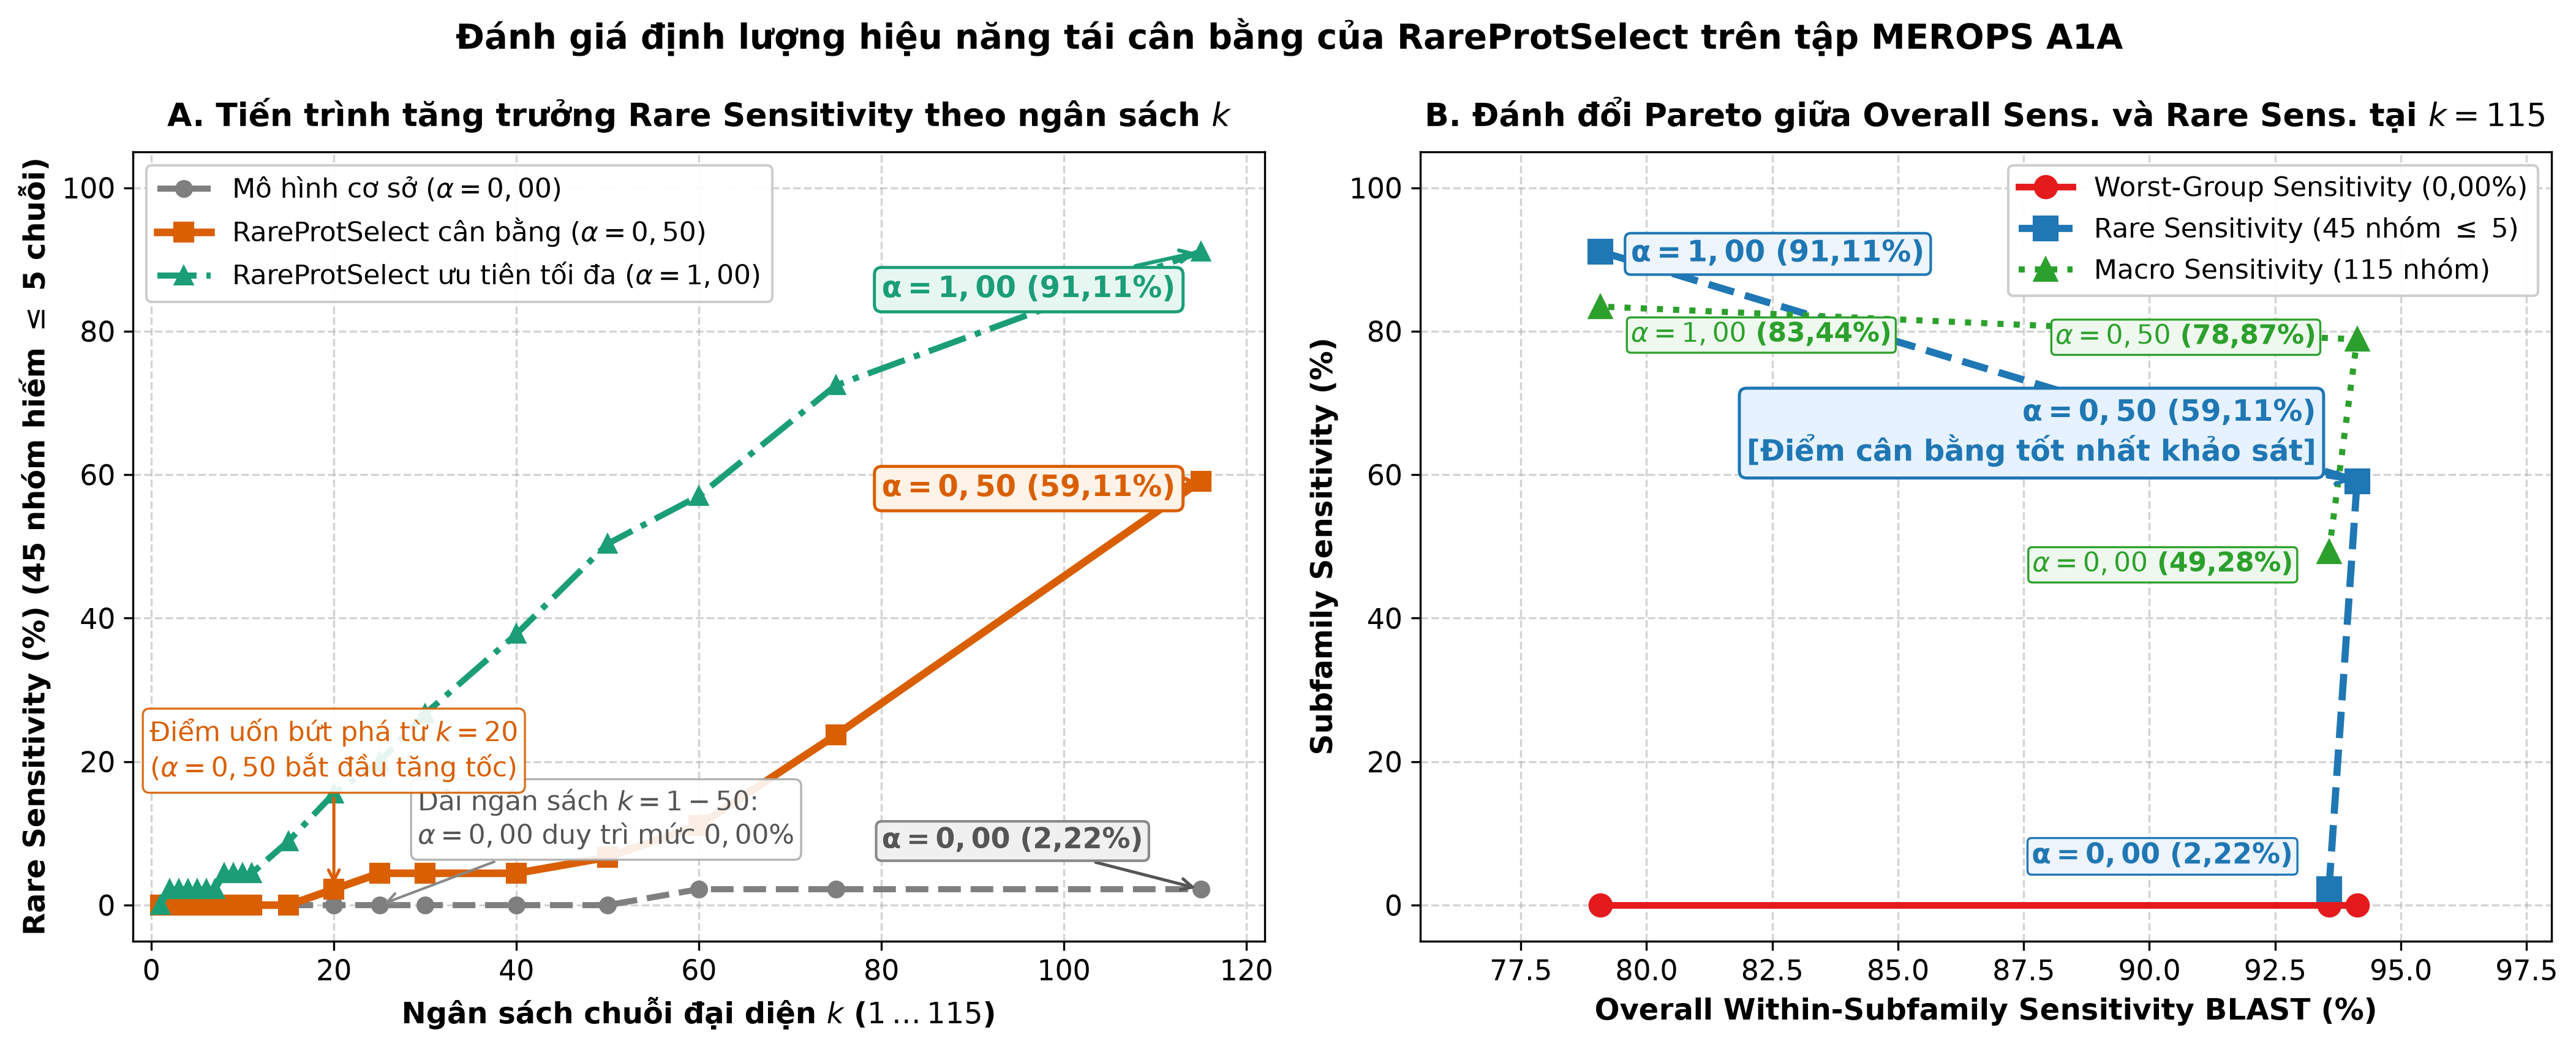
\includegraphics[width=0.68\textwidth]{Images/figures/exp2_pareto_tradeoff.png}
    \vspace{-6pt}
    \caption{Đánh giá hiệu năng của RareProtSelect trên tập MEROPS A1A: (A) Tiến trình Rare Sensitivity theo ngân sách $k \in [1, 115]$; (B) Đánh đổi Pareto giữa Overall Sensitivity và Subfamily Sensitivity tại $k = 115$.}
    \label{fig:exp2_pareto}
    \vspace{-6pt}
\end{figure}

Đồ thị tại hình~\ref{fig:exp2_pareto} phản ánh rõ nét hai góc nhìn phương pháp luận:
\begin{itemize}[noitemsep,topsep=1pt]
    \item \textbf{Tiến trình theo ngân sách (Hình~\ref{fig:exp2_pareto}A)}: mô hình cơ sở $\alpha = 0{,}00$ duy trì Rare Sensitivity xấp xỉ $0\%$ suốt dải $k = 1 - 50$ và chỉ đạt $2{,}22\%$ tại $k = 115$. Trong khi đó, RareProtSelect $\alpha = 0{,}50$ tăng tốc từ mốc $k = 20$ và đạt $59{,}11\%$ tại $k = 115$, còn $\alpha = 1{,}00$ đạt $91{,}11\%$.
    \item \textbf{Đánh đổi Pareto tại $k = 115$ (Hình~\ref{fig:exp2_pareto}B)}: Tại $k = 115$, cấu hình $\alpha = 0{,}50$ đạt giá trị cao hơn mô hình cơ sở $\alpha = 0{,}00$ trên cả ba chỉ số: Overall Sensitivity đạt $94{,}13\%$ so với $93{,}57\%$, Macro-Average Sensitivity đạt $78{,}87\%$ so với $49{,}28\%$ và Rare Sensitivity đạt $59{,}11\%$ so với $2{,}22\%$, xác lập điểm cân bằng tốt nhất trong ba cấu hình khảo sát.
\end{itemize}

\section{Kiến trúc kỹ thuật và công nghệ triển khai tại ORLab}
\label{sec:kien_truc_cong_nghe}

Hệ thống mã nguồn của đề tài được đóng gói chuẩn mực trong thư mục \textbf{RareProtSelect/}:
\begin{itemize}[noitemsep,topsep=0pt,partopsep=0pt]
    \item \textbf{Môi trường và trình quản lý gói}: Quản lý môi trường ảo độc lập qua công cụ uv trên nền Python 3.12, bảo đảm tốc độ cài đặt và tính tái lập chuẩn xác.
    \item \textbf{Tăng tốc tính toán phần cứng}: bộ xử lý AMD Ryzen 9 8940HX ($16$ nhân, $32$ luồng) kết hợp GPU NVIDIA RTX 5060 ($8\text{ GB}$ GDDR6, CUDA 13.0). Phép trích xuất embedding ESM-2 và tính toán ma trận thực thi trực tiếp trên GPU.
    \item \textbf{Cấu hình thí nghiệm tự động}: Sử dụng các tệp cấu hình YAML phân tách rõ ràng giữa tham số mô hình $\alpha, \beta, k$, đường dẫn dữ liệu và kịch bản thực nghiệm, phục vụ quy trình chạy hàng loạt ổn định.
\end{itemize}

\chapter{TỰ ĐÁNH GIÁ}
\label{chap:tu_danh_gia}

Sau 3 tuần thực tập (từ ngày 26/10/2026 đến ngày 15/11/2026) và trực tiếp tham gia nghiên cứu đề tài tại phòng thí nghiệm ORLab, tôi tự đánh giá các kết quả đạt được, năng lực cá nhân cũng như những trải nghiệm học thuật trong môi trường nghiên cứu chuyên sâu.

\section{So với mục tiêu ban đầu}
\label{sec:danh_gia_muc_tieu}

Đối chiếu với các mục tiêu cá nhân và nhiệm vụ nghiên cứu khoa học đã đề ra trong chương~\ref{chap:ke_hoach_lich_trinh}, tôi đã hoàn thành đầy đủ các cam kết học thuật:

\begin{itemize}
    \item \textbf{Về mặt khoa học và mô hình hóa}: Đã hoàn thiện mô hình toán học RareProtSelect, chứng minh chặt chẽ tính đơn điệu không giảm và submodular của hàm mục tiêu Facility Location có trọng số phạt quy mô nhóm, bảo đảm tỷ lệ xấp xỉ $(1 - 1/e)$ theo định lý Nemhauser.
    \item \textbf{Về mặt kỹ thuật và giải thuật}: Đã cài đặt thành công thuật toán tham lam cắt tỉa Pruned Greedy 90\% tăng tốc trên GPU PyTorch CUDA và cơ chế tổng hợp thứ hạng toàn cục qua $1.000$ lần xáo trộn ngẫu nhiên. Đồng thời, giải quyết thành công hiện tượng co cụm vector Anisotropy của mô hình ngôn ngữ protein ESM-2 bằng kỹ thuật dịch tâm Mean-Centering.
    \item \textbf{Về mặt thực nghiệm và sản phẩm bàn giao}: Đã chạy thực tế $100\%$ cả 6 kịch bản thử nghiệm đối chuẩn trên tập $4.120$ chuỗi MEROPS A1A, lưu trữ dữ liệu định lượng nguyên văn vào các tệp CSV và đồ thị đạt chuẩn xuất bản học thuật.
\end{itemize}

\section{Tự đánh giá hiệu suất trong quá trình thực tập}
\label{sec:danh_gia_hieu_suat}

Tôi luôn duy trì tinh thần làm việc chủ động, nghiêm túc tuân thủ lịch trình và các quy chuẩn kỹ thuật tại ORLab:
\begin{itemize}
    \item \textbf{Tính kỷ luật và đúng hạn}: Toàn bộ các mốc công việc từ khảo sát lý thuyết, thiết kế pipeline đến đo đạc thực nghiệm đều được hoàn thành đúng hoặc sớm hơn thời hạn trong kế hoạch tuần.
    \item \textbf{Khả năng giải quyết nút thắt kỹ thuật}: Trong quá trình tính toán ma trận tương đồng trên dữ liệu lớn, khi gặp thách thức về chi phí thời gian và sự phụ thuộc vào thứ tự duyệt mảng khi các ứng viên có cùng độ tăng cận biên, tôi đã chủ động đề xuất giải pháp vector hóa giải thuật Pruned Greedy 90\% trên GPU PyTorch CUDA kết hợp cơ chế tổng hợp thứ hạng toàn cục qua $1.000$ vòng xáo trộn hoán vị ngẫu nhiên để bảo đảm hiệu năng tính toán và độ ổn định của mã nguồn.
    \item \textbf{Ý thức liêm chính khoa học}: Tuân thủ nghiêm ngặt nguyên tắc đối soát dữ liệu nguyên văn $100\%$, tuyệt đối không suy diễn hay đưa ra các số liệu giả định trong báo cáo kỹ thuật.
\end{itemize}

\section{Tự đánh giá kỹ năng cá nhân}
\label{sec:danh_gia_ky_nang}

Kỳ thực tập tại ORLab đã mang lại sự trưởng thành vượt bậc cho tôi trên cả phương diện kỹ thuật chuyên môn lẫn phương pháp luận nghiên cứu:

\subsection{Kỹ năng kỹ thuật và lập trình}
\begin{itemize}
    \item Thành thạo việc xây dựng kiến trúc codebase nghiên cứu hoàn chỉnh bằng Python 3.12 và trình quản lý môi trường hiện đại uv.
    \item Nâng cao năng lực tính toán khoa học với PyTorch tăng tốc trên GPU NVIDIA CUDA 13.0, tối ưu hóa các phép toán đại số tuyến tính trên ma trận lớn.
    \item Làm chủ các công cụ tin sinh học phân tử như Biopython, BLASTp cục bộ và mô hình ngôn ngữ protein ESM-2 của Meta AI.
\end{itemize}

\subsection{Kỹ năng mềm và phương pháp luận nghiên cứu}
\begin{itemize}
    \item Rèn luyện tư duy tiếp cận bài toán theo nguyên tắc cô lập biến số và phương pháp luận so sánh đối chứng khoa học khách quan.
    \item Kỹ năng đọc hiểu, tổng hợp và phản biện các bài báo khoa học quốc tế uy tín trong các lĩnh vực tối ưu hóa tổ hợp và tin sinh học.
    \item Năng lực soạn thảo văn bản học thuật chuyên nghiệp bằng LaTeX với hệ thống ký hiệu toán học giải tích chặt chẽ, quản lý tài liệu tham khảo và bảng biểu chuẩn mực.
\end{itemize}

\section{Đánh giá về chương trình thực tập}
\label{sec:danh_gia_moi_truong_orlab}

Tôi đánh giá rất cao môi trường học thuật và nghiên cứu tại phòng thí nghiệm ORLab:
\begin{itemize}
    \item \textbf{Sự định hướng chuyên sâu và tâm huyết}: TS. Trần Đình Tân luôn theo sát tiến độ nghiên cứu, đặt ra những câu hỏi phản biện sâu sắc giúp tôi nhìn nhận rõ bản chất toán học và cơ chế vận hành của mô hình.
    \item \textbf{Môi trường cởi mở và khuyến khích sáng tạo}: Lab tạo mọi điều kiện thuận lợi về tài nguyên tính toán, tài liệu học thuật và không gian trao đổi để tôi tự do thử nghiệm các ý tưởng giải thuật mới.
    \item \textbf{Tính thực tế và kết nối liên ngành}: Đề tài thực tập không chỉ dừng lại ở lý thuyết thuần túy mà gắn liền trực tiếp với bài toán lớn trong sinh học phân tử, mở ra triển vọng phát triển thành các công bố khoa học quốc tế có giá trị thực tiễn.
\end{itemize}

\chapter{KẾT LUẬN VÀ KIẾN NGHỊ}
\label{chap:ket_luan_kien_nghi}

Chương này tổng kết toàn bộ các kết quả đạt được trong đợt thực tập công nghiệp tại phòng thí nghiệm ORLab, đề xuất các hướng phát triển nghiên cứu tiếp theo cho đề tài RareProtSelect và đưa ra các kiến nghị mang tính xây dựng nhằm nâng cao chất lượng chương trình thực tập.

\section{Tổng kết công việc thực tập}
\label{sec:tong_ket_thuc_tap}

Kỳ thực tập công nghiệp tại phòng thí nghiệm ORLab đã giúp tôi hoàn thành xuất sắc các mục tiêu học thuật và nhiệm vụ kỹ thuật được giao:
\begin{enumerate}
    \item \textbf{Khắc phục hạn chế phương pháp luận}: Đã phát hiện và giải quyết thành công điểm mù thiên lệch quy mô mẫu của các phương pháp chọn protein đại diện truyền thống trên phân bố đuôi dài Long-Tail.
    \item \textbf{Đóng góp mô hình toán học}: Xây dựng thành công mô hình submodular Facility Location có trọng số phạt quy mô nhóm $w_v^{(\alpha)} = (n_g)^{-\alpha}$ với bảo đảm chặn cận giải tích chặt chẽ $(1 - 1/e)$ theo định lý Nemhauser.
    \item \textbf{Kết quả đối chuẩn chỉ số thực nghiệm}: Trên tập dữ liệu thực nghiệm trọng tâm MEROPS A1A gồm $4.120$ chuỗi thuộc $115$ Subfamily, phương pháp RareProtSelect giúp cải thiện rõ rệt tính đại diện nhóm hiếm: tại $k = 115$, cấu hình $\alpha = 0{,}50$ nâng Rare Sensitivity từ $2{,}22\%$ lên $59{,}11\%$ và $\alpha = 1{,}00$ đạt tới $91{,}11\%$, đồng thời cắt giảm số Subfamily có Zero-Sensitivity Count từ $58$ xuống còn $18$, khắc phục hiệu quả điểm mù bỏ sót Subfamily hiếm của phương pháp truyền thống.
    \item \textbf{Đóng gói sản phẩm hoàn chỉnh}: hệ thống mã nguồn được xây dựng bài bản bằng Python 3.12, quản lý qua uv, tăng tốc tính toán trên GPU CUDA và lưu trữ toàn bộ dữ liệu thực nghiệm minh bạch, có thể tái~lập~$100\%$.
\end{enumerate}

\section{Kế hoạch tương lai}
\label{sec:ke_hoach_tuong_lai}

Trên nền tảng các kết quả đã đạt được trong kỳ thực tập, tôi dự kiến tiếp tục hợp tác cùng ORLab để phát triển đề tài theo các định hướng:
\begin{itemize}
    \item \textbf{Đánh giá tính tổng quát hóa trên quy mô siêu lớn}: triển khai đối chuẩn mở rộng trên tập dữ liệu CE.fasta gồm $12.277$ chuỗi từ cơ sở dữ liệu ESTHER, đồng thời nghiên cứu mở rộng thuật toán Lazy Greedy với cấu trúc Max-Heap để tối ưu hóa thời gian tính toán trên các siêu họ enzyme có quy mô trên $10.000$ chuỗi.
    \item \textbf{Tích hợp thông tin cấu trúc không gian 3 chiều}: Khai thác các ma trận tương đồng cấu trúc dựa trên tọa độ nguyên tử từ AlphaFold2 hoặc ESMFold để bổ sung cho thông tin trình tự sơ cấp.
    \item \textbf{Công bố công trình khoa học}: Hoàn thiện bản thảo bài báo khoa học dựa trên phương pháp luận RareProtSelect để gửi đăng tại các hội thảo hoặc tạp chí quốc tế uy tín trong danh mục ISI/Scopus thuộc lĩnh~vực~vận~trù~học và tin~sinh~học~tính~toán.
\end{itemize}

\section{Kiến nghị}
\label{sec:kien_nghi}

Từ những trải nghiệm thực tế trong kỳ thực tập, tôi xin đề xuất một số kiến nghị nhằm nâng cao hiệu quả đào tạo và nghiên cứu:

\subsection{Đối với nhà trường và khoa}
\begin{itemize}
    \item Tiếp tục đẩy mạnh mô hình gắn kết đào tạo lý thuyết với thực hành nghiên cứu tại các phòng thí nghiệm chuyên sâu theo định hướng Lab-based learning ngay từ các năm học đầu.
    \item Đầu tư và mở rộng hạ tầng máy chủ tính toán hiệu năng cao với các cụm GPU để hỗ trợ sinh viên thực hiện các đề tài trí tuệ nhân tạo và xử lý dữ liệu lớn.
    \item Tổ chức thêm các hội thảo học thuật định kỳ để sinh viên các nhóm nghiên cứu có cơ hội giao lưu, chia sẻ phương pháp luận và kết quả thực nghiệm.
\end{itemize}

\subsection{Đối với cơ sở thực tập ORLab}
\begin{itemize}
    \item Tiếp tục phát huy thế mạnh về môi trường học thuật nghiêm túc, cởi mở và phương pháp hướng dẫn tận tâm, sát sao đối với sinh viên thực tập.
    \item Mở rộng kết nối và hợp tác liên ngành với các viện nghiên cứu sinh học phân tử thực nghiệm nhằm tạo điều kiện cho các thuật toán tối ưu hóa được kiểm chứng in vitro trong phòng thí nghiệm sinh học.
\end{itemize}

\subsection{Đối với sinh viên các khóa tiếp theo}
\begin{itemize}
    \item Cần chủ động trang bị nền tảng toán học giải tích, lý thuyết xác suất và kỹ năng lập trình khoa học từ sớm trước khi bước vào kỳ thực tập công nghiệp.
    \item Rèn luyện tác phong kỷ luật, tư duy phản biện và tinh thần tự học, chủ động trao đổi thường xuyên với cán bộ hướng dẫn để tháo gỡ kịp thời các khó khăn phát sinh trong quá trình nghiên cứu.
\end{itemize}


% 7. Tài liệu tham khảo
\clearpage
\phantomsection
\addcontentsline{toc}{chapter}{TÀI LIỆU THAM KHẢO}

\begingroup
\setstretch{1.05}
\begin{thebibliography}{99}
\raggedright
\setlength{\itemsep}{1pt}
\setlength{\parskip}{0pt}

\bibitem{nguyen2025}
H. Nguyen, et al.,
\textit{Identifying representative sequences of protein families using submodular optimization},
Scientific Reports, vol. 15, art. no. 1069, 2025. doi: 10.1038/s41598-025-85165-1.

\bibitem{esm2}
Z. Lin, H. Akin, R. Rao, B. Hie, Z. Zhu, W. Lu, N. Smetanin, R. Verkuil, O. Kabeli, Y. Shmueli, et al.,
\textit{Evolutionary-scale prediction of atomic-level protein structure with a language model},
Science, vol. 379, no. 6637, pp. 1123-1130, 2023.

\bibitem{blast}
S. F. Altschul, W. Gish, W. Miller, E. W. Myers, and D. J. Lipman,
\textit{Basic local alignment search tool},
Journal of Molecular Biology, vol. 215, no. 3, pp. 403-410, 1990.

\bibitem{camacho2009}
C. Camacho, G. Coulouris, V. Avagyan, N. Ma, J. Papadopoulos, K. Bealer, and T. L. Madden,
\textit{BLAST+: architecture and applications},
BMC Bioinformatics, vol. 10, no. 1, p. 421, 2009.

\bibitem{merops}
N. D. Rawlings, M. Waller, A. J. Barrett, and A. Bateman,
\textit{MEROPS: the database of proteolytic enzymes, their substrates and inhibitors},
Nucleic Acids Research, vol. 42, no. D1, pp. D503-D509, 2014.

\bibitem{nemhauser1978}
G. L. Nemhauser, L. A. Wolsey, and M. L. Fisher,
\textit{An analysis of approximations for maximizing submodular set functions - I},
Mathematical Programming, vol. 14, no. 1, pp. 265-294, 1978.

\bibitem{minoux1978}
M. Minoux,
\textit{Accelerated greedy algorithms for maximizing submodular set functions},
Optimization Techniques, Lecture Notes in Control and Information Sciences, vol. 7, pp. 234-243, Springer, 1978.

\bibitem{wei2015}
K. Wei, R. K. Iyer, and J. A. Bilmes,
\textit{Submodularity in data subset selection and active learning},
in Proceedings of the 32nd International Conference on Machine Learning (ICML), pp. 1954-1963, 2015.

\bibitem{cui2019}
Y. Cui, M. Jia, T.-Y. Lin, Y. Song, and S. Belongie,
\textit{Class-balanced loss based on effective number of samples},
in Proceedings of the IEEE/CVF Conference on Computer Vision and Pattern Recognition (CVPR), pp. 9268-9277, 2019.

\bibitem{ethayarajh2019}
K. Ethayarajh,
\textit{How contextual are contextualized word representations? Comparing the geometry of BERT, ELMo, and GPT-2 embeddings},
in Proceedings of EMNLP-IJCNLP, pp. 55-65, 2019.

\bibitem{cdhit}
W. Li and A. Godzik,
\textit{Cd-hit: a fast program for clustering and comparing large sets of protein or nucleotide sequences},
Bioinformatics, vol. 22, no. 13, pp. 1658-1659, 2006.

\bibitem{mmseqs2}
M. Steinegger and J. S\"oding,
\textit{MMseqs2 enables sensitive protein sequence searching for the analysis of massive data sets},
Nature Biotechnology, vol. 35, no. 11, pp. 1026-1028, 2017.

\end{thebibliography}
\endgroup

\clearpage


\end{document}
